\chapter{Method}

This project consists of a series of trials aimed at evaluating different aspects of the fitting process. Each trial involves first simulating and fitting multiple spectra, then analysing the results of the fits. The former was accomplished using the PALSfit software package and the associated PALSsim program, while for the latter custom Python scripts were written to group the fits together and create relevant plots, using the Matplotlib library.

Each trial can be further grouped into one of three categories. The first investigates how changing the lifetimes and intensities of a two lifetime spectrum affects the fit. The second looks at experimental parameters, in particular what can be changed about PALS experiments to improve fitting performance. The third focuses on modeling spectra that closer reflect real experimental spectra.

In this chapter is a description and overview of the tools used to generate, fit and analyse the spectra that make up each trial.

\section{The PALSfit Bundle}

PALSfit is a Windows based software package, developed for the analysis of positron lifetime spectra, based on a non-linear least squares approach. Included are two modules, POSITRONFIT and RESOLUTIONFIT, which are used to deconvolve the lifetime components and resolution functions (respectively) from the lifetime spectra. As the scope of the project limited to lifetime component analysis, only the former will be used. PALSfit Version 3, or more simply PALSfit3, is the latest version of this package, which this project is aimed at evaluating. All subsequent references to "PALSfit" are to this specific version of the software.

Included with PALSfit is the PALSsim program, which generates lifetime spectra based on user input. PALSsim makes it possible to quickly generate spectra with full control over relevant parameters such as lifetimes, resolution function, background noise, etc. All spectra to be analysed in the project were produced using PALSsim.

\subsection{PALSsim}
\begin{figure}
     
    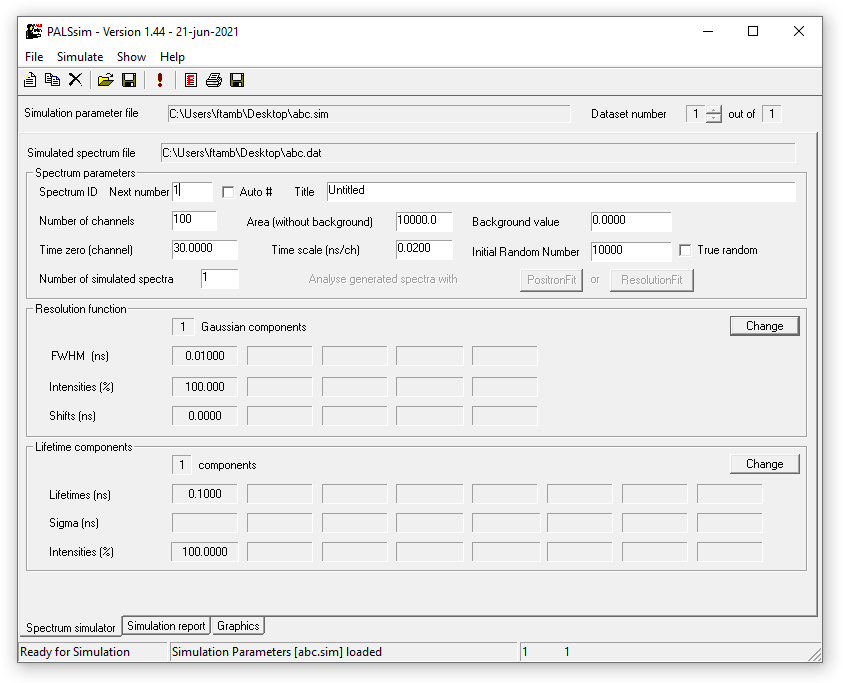
\includegraphics[width=0.8\linewidth]{PALSsim.PNG}
    \caption{PALSsim window}
    \label{fig:Psim}
\end{figure}

As can be seen in Fig.\ref{fig:Psim}, PALSsim groups user input data into three sections: Spectrum parameters, Resolution function and Lifetime components.

In the \textit{Lifetime components} section, the number of components in the spectrum and their associated values can be modified. Only the \textit{Lifetimes} and \textit{Intensities} fields will be used for each component throughout this project, as we'll assume each lifetime component to be discrete. Up to eight components can be simulated, but the maximum number of components used in the project will be three.

The \textit{Resolution function} section deals with the instrument resolution function of the simulated spectrum. The resolution function is given by a sum of up to five Gaussian functions $G(t)$ with the width, relative height and peak position of each Gaussian component being controlled by the \textit{FWHM}, \textit{Intensities} and \textit{Shifts fields} respectively.

For the majority of this project, a three gaussian resolution function will be used, with the appropriate parameters taken from an experimental spectrum and indicated in Table \ref{tab:irfcomp}. For a visual representation of the IRF, see Fig. \ref{fig:irf}.

The variables found within the \textit{Simulation parameters} section affect the spectrum as a whole. Here we find parameters controlling the number of channels, time per channel, number of counts, $t_0$ and background noise. Relevant parameters and default values used are as follows:

\begin{itemize}
    \item Number of channels: 1000 
    \item Area (without background): 5650000 
    \item Background value: 8.5 
    \item Time zero (channel): 1400 
    \item Time scale (ps/ch): 5 
\end{itemize}
All other parameters were left unchanged.

PALSsim generates five files every time a new spectrum is simulated. The file with the .dat extension contains the simulated spectrum, organized as a table of values for each channel. A .sim file stores the simulated values, allowing them to be reloaded into the program. A simulation report is generated every time a simulation is ran that contains data about the spectrum and saved in a .out file. Lastly two control files with the .pfc and .rfc extensions are generated to be read by PALSfit. Loading one or the other control file into PALSfit determines whether the POSITRONFIT or RESOLUTIONFIT module is used to analyse the spectrum (.pfc for the former and .rfc for the latter).

\begin{minipage}{0.6\textwidth}
    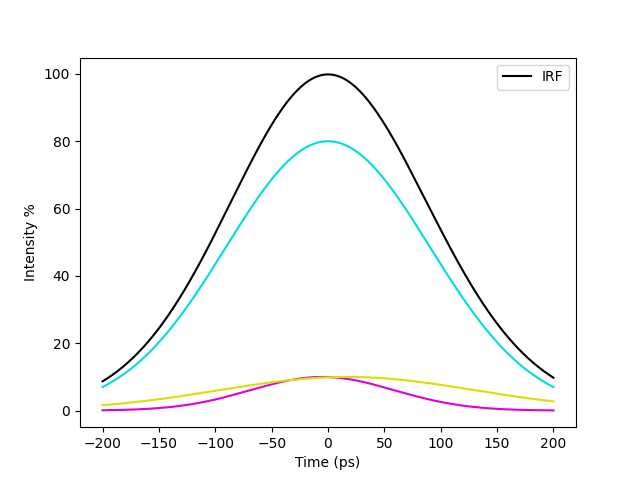
\includegraphics[width=\textwidth]{Batch 3/regular IRF/irf.png}
\end{minipage}
\begin{minipage}{0.35\textwidth}
     
    \captionof{table}{IRF values}
    \label{tab:irfcomp}
    \begin{tabular}{|c|c|c|}
        \hline
        FWHM& Intensity& Shift \\
        (ps) & (\%) & (ps)\\
        \hline
        213.2 & 80 &  0\\
        150.2 & 10 & -5\\
        265.7 & 10 & 17\\
        \hline
    \end{tabular}
    \vspace{1cm}
    \captionof{figure}{Visual representation of the IRF, generated using Python and Matplotlib}
    \label{fig:irf}
\end{minipage}

\subsection{PALSfit}

Opening a .pfc file with PALSfit should automatically load the spectrum and all relevant fitting values. The \textit{Spectrum setup} window can be opened by clicking any of the two \textit{Change} buttons in the \textit{Spectrum} tab (selected by default when the program is opened). Here the \textit{Default Ranges} button can be clicked to ensure that the appropriate range is fitted and the spectrum can be saved to the control file by checking the relevant checkbox.

\vfill

\begin{figure}[h]
     
    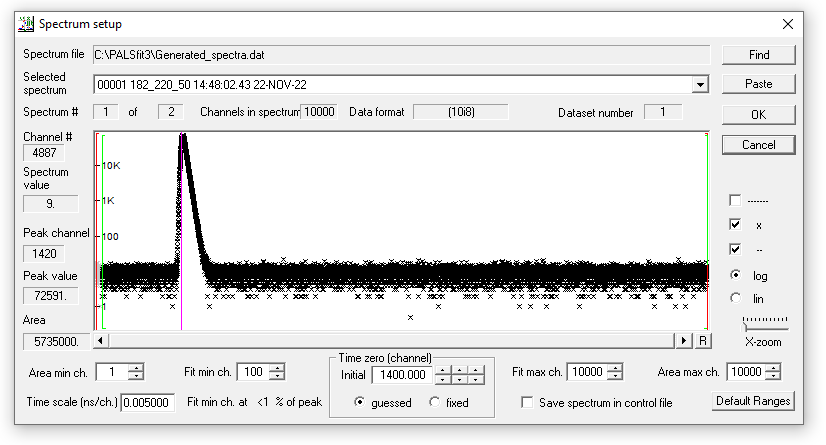
\includegraphics[width=0.6\linewidth]{SpecSetup.PNG}
    \caption{Spectrum setup window}
    \label{fig:SpecSet}
\end{figure}

Seven other tabs are present at the bottom of the program. The \textit{Resolution function} tab shows a graphical representation of the resolution function used during fitting, and allows the user to modify the Gaussian components that make up the IRF. In the \textit{Lifetime and Corrections} tab, the number of lifetime components and the initial values used in fitting them can be modified. Meanwhile, the \textit{Text output} tab displays the result of the last fit. All other tabs can be safely ignored, at least in the context of this project.

A fit is performed by pressing the \textit{Analyse} button at the top of the window or pressing the F5 key. This generates a series of files in an output folder, contained in the same directory as the .pfc file. Of relevance are the .out file and .csv file that contain the results of the fit.

\section{Python Scripts}

Custom Python scripts were developed for the following purposes:

\subsection{Grouping fit results}
As each trial involves generating and fitting multiple spectra, the results of multiple fits had be collected into a single document for analysis. To this end, files were grouped into batches and subfolders containing spectra to be analysed together. Once generated and fitted, the fit results for each subfolder were contained in a single output folder. Two Python scripts were initially used to collect the data into a single file with all relevant information for plotting, that later were consolidated into one. The first script joined the multiple .csv files produced by PALSfit and the second added information on the original, simulated values of the lifetime components to the file.

\subsection{Plotting fit data}

All plots were produced using Python library Matplotlib. These can be grouped into a few different types, with an overview provided below as a reference to aid in interpretation.

An example of the first type, used for two-lifetime spectra, can be seen in Figure \ref{fig:type1}. On the x-axis is always the simulated value of $\tau_2$. On the y-axis is either $\tau_1$, with the (fixed) simulated value of $\tau_1$ indicated with a grey dashed line, or the difference between the fitted and simulated values of $\tau_2$, with the grey line at $y=0$. Each datapoint represents a different spectrum. For each simulated $\tau_2$, there are three datapoints, indicating the relative intensities of the two lifetime components, marked in the legend. Error bars are given by the standard deviation calculated by PALSfit.

\begin{minipage}{0.46\textwidth}
     
    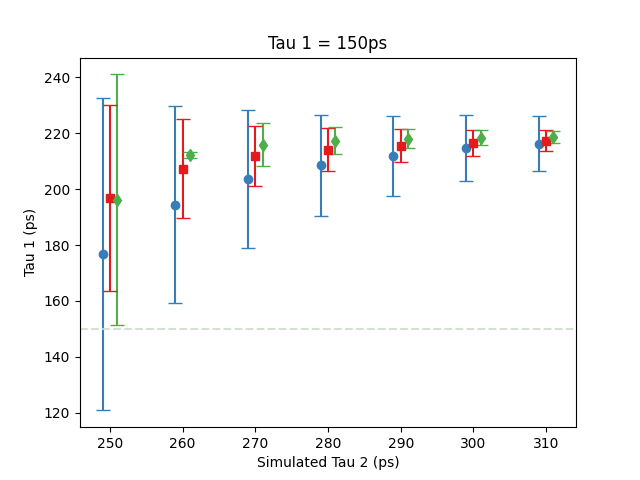
\includegraphics[width=\textwidth]{Batch 3/regular IRF/tau1 220/output/t1.png}
    \captionof{figure}{$\tau_1$ = 220 ps (fixed), $\tau_2$ = 260-320 ps}
    \label{fig:type1}
\end{minipage}
\hfill
\begin{minipage}{0.46\textwidth}
     
    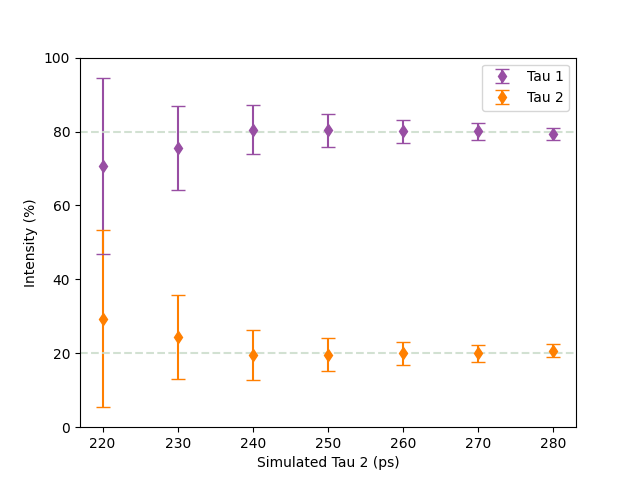
\includegraphics[width=\textwidth]{Batch 1+2/8020.png}
    \captionof{figure}{$I_1:I_2 = 80\%:20\%$, $\tau_2$ = 260-320 ps}
    \label{fig:type2}
\end{minipage}

Closely related is the second type, shown in Figure \ref{fig:type2} and also used for two-lifetime fits. The simulated $\tau_2$ is still on the x-axis, but lifetime intensity is on the y-axis, instead. The grey lines trace the simulated values for $I_1$ and $I_2$ and each spectrum is represented by two vertically stacked points, representing the fitted values of $I_1$ and $I_2$, as indicated in the legend.

\begin{figure}[h]
     
    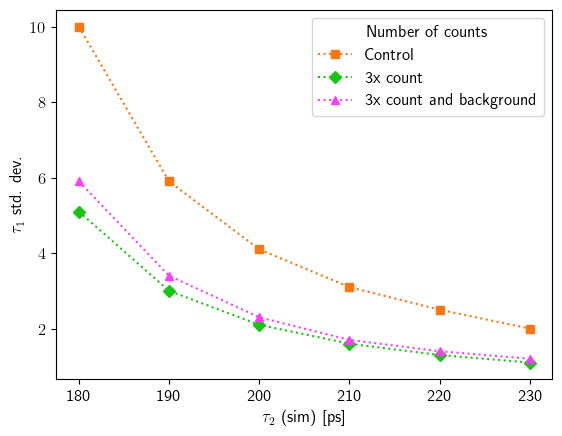
\includegraphics[width=0.6\linewidth]{Batch 5/t1-err 5050.png}
    \caption{Std. dev. $\tau_1$, $I_1:I_2 = 50\%:50\%$}
    \label{fig:type3}
\end{figure}

In the third type a single fit result is being tracked on the y-axis, across the same intensity ratio, and with the x-axis representing (again) simulated $\tau_2$. Figure \ref{fig:type3} is an example where the variable being tracked is the standard deviation of $\tau_1$, the intensity ratio is 50\%-50\%, and each colored line represents a different number of counts in the spectrum, indicated in the legend. Like the first type, each datapoint corresponds to an individual spectrum. Each spectrum is made up of two lifetime components, as in the previous types.

 
\begin{minipage}{.47\linewidth}
     
    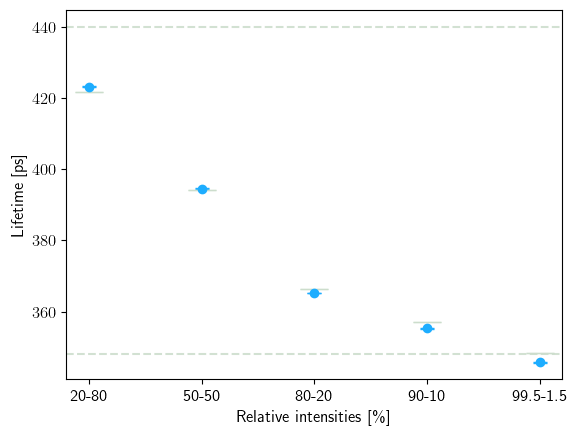
\includegraphics[width=\linewidth]{Batch 7/348-440/output/1 life/lifetimes.png}
    \captionof{figure}{One lifetime fit, $\tau_1=348$ps, $\tau_2=440$ps}
    \label{fig:type4a}
\end{minipage}
\hfill
\begin{minipage}{.47\linewidth}
     
    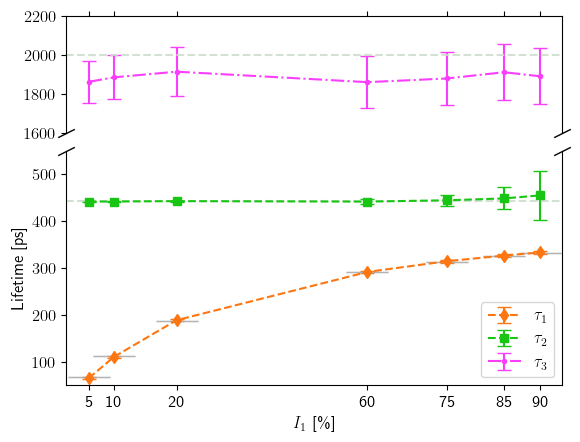
\includegraphics[width=\linewidth]{Batch 8/442/output/lifetimes.png}
    \captionof{figure}{Three lifetime fit, Standard trapping model, $\tau_b=339$ps, $\tau_d=442$ps}
    \label{fig:type4b}
\end{minipage}
 

For tracking multiple lifetimes across a range of intensities, the fourth type will be used. This has intensity on the x-axis, and on the y-axis is lifetime. Grey dashed lines indicate important fixed values. Short grey lines are used to indicate a value being compared against. In Figure \ref{fig:type4a}, for example, the dashed line indicate two lifetimes and the short grey lines represent the intensity-weighted average lifetime. In Figure \ref{fig:type4a}, the short grey lines indicate the reduced bulk lifetime.



\subsection{Generating a single Gaussian resolution function\label{singlegauss}}
As one of the trials requires varying the width of the resolution function, a script was developed to approximate the three Gaussian resolution function used throughout the paper (see Table \ref{tab:irfcomp}) with a single Gaussian resolution function. This same script was also used to produce Figure \ref{fig:irf}. Outlined is the procedure used.
The equation for a Gaussian function with parameters $a$, $b$ and $c$ (corresponding to the height of the peak, the position of the peak and the width of the graph) is given by the equation:
\begin{equation}
    g(x) = a\exp{\left[-\frac{-(x-b)^2}{2c^2}\right]}
\end{equation}
While $a$ and $b$ map easily to the intensity and shift columns in Table \ref{tab:irfcomp},  $c$ is expressed as a standard deviation, and not the full-half-width-maximum given in the table. To convert from one to the other, the following expression was used:
\begin{equation}
    \mathrm{FWHM} = 2\sqrt{2\ln(2)} \approx 2.355c
\end{equation}
giving the resulting resolution function
\begin{equation}
    g_s(x) = \sum_{i=1}^{3}{a_i \exp{\left(-\frac{(x-b)^2}{2c^2}\right)}}
    \label{eq:composite-res}
\end{equation}
As this is a single Gaussian resolution function, intensity is simply 100\%. FWHM and shift can be determined analytically, by solving eq. {eq:composite-res}, but as a plot of $g_s(x)$ would be generated for use in this document, the choice was made to just extract these variables numerically using Python.
To find the shift, the largest $y$-value was picked and its corresponding $x$-value was found. To find the FWHM the difference was calculated between the two values of $x$ for which $g_s(x)$ is closest to half of the IRF.
The resulting resolution function has a FWHM of $\sim$210 ps and a shift of $\sim$0 ps.

\subsection{Batch simulation and fitting}
A command-line version of PALSfit called PATFIT is available for use, found on the PALSfit website, as an auxiliary program. By using a Python library for interfacing with command-line programs, a script was developed that uses PATFIT to fit multiple spectra. This script then takes the .csv files produced by these fits and groups them into a single file. A separate script was also developed that allows for multiple .sim files to be generated, which can then be simulated using PALSsim.
Using these two scripts still requires the user to simulate each .sim file individually, then link the spectrum file and adjust the fitting ranges on PALSfit. This can be tedious, however, and a single script to automate the entire process could be both useful and possible to code, though deemed beyond the scope of this project.